\documentclass[12pt,aspectratio=169]{beamer}

\usetheme[
    sectionpage=progressbar,
    subsectionpage=progressbar,
    progressbar=frametitle
]{metropolis}

\usefonttheme{professionalfonts}

\definecolor{blue-grey-900}{HTML}{263238}
\definecolor{deep-orange-500}{HTML}{FF5722}
\setbeamercolor{normal text}{fg=blue-grey-900, bg=white}
\setbeamercolor{alerted text}{fg=deep-orange-500}

\usepackage{booktabs}
\usepackage{graphicx}
\usepackage{hyphenat}
\usepackage{multirow}

\usepackage{polyglossia}
\setdefaultlanguage[variant=british]{english}
\usepackage[english=british]{csquotes}

\usepackage{fontspec}
\setmainfont{Lucida Sans OT}
\setsansfont[Scale=MatchLowercase]{Lucida Sans OT}
\setmonofont[Scale=MatchLowercase]{Lucida Console DK}
\defaultfontfeatures{Ligatures=TeX}

\usepackage{mathspec}
\setmathsfont(Digits,Latin,Greek)[Numbers={Lining,Proportional}]{Lucida Bright Math OT}

\author{Gianluca Campanella}
\title{Data Science for Scientists}
\date{17\textsuperscript{th} July 2018}



\subtitle{The what, why and how of Data Science}

\begin{document}

\maketitle

\begin{frame}
    \only<1>{%
        \begin{center}
            \LARGE%
            What is Data Science?
        \end{center}}
    \only<2>{%
        \begin{center}
            \LARGE%
            When did Data Science start?
        \end{center}}
    \only<3>{%
        \begin{center}
            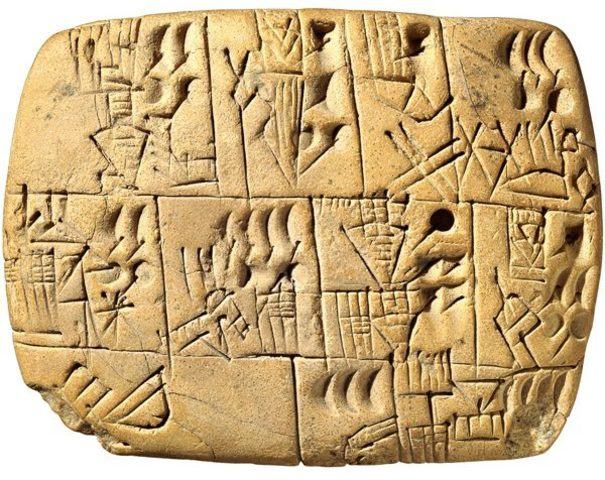
\includegraphics[height=0.8\textheight]{figures/counting_beer} \\
            {\scriptsize%
             From the British Museum collection}
        \end{center}}
    \only<4>{%
        \begin{center}
            \LARGE%
            So\ldots \\
            What is Data Science?
        \end{center}}
\end{frame}

\begin{frame}{What is Data Science?}
    \begin{center}
        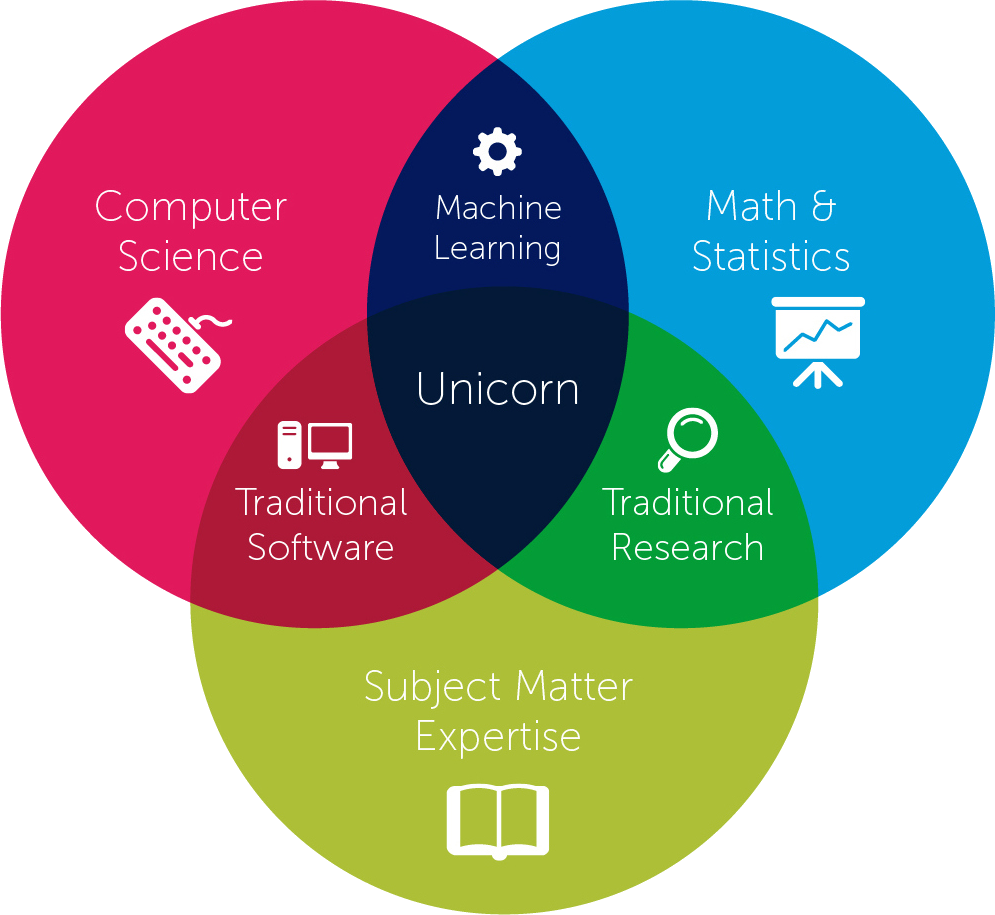
\includegraphics[height=0.8\textheight]{figures/data_science_venn_diagram} \\
        {\scriptsize%
         From S.\ Geringer (originally from D.\ Conway)}
    \end{center}
\end{frame}

{\setbeamertemplate{background}{%
    \rule{0.5\paperwidth}{0pt}%
    \rule{0pt}{\paperheight}%
    
\includegraphics[height=0.5\paperheight]{figures/confused_cat}}
\begin{frame}{How's it different from\ldots}
    \begin{itemize}
        \item Applied Mathematics?
        \item Statistics?
        \item Operational Research?
        \item Business Intelligence?
        \item Predictive Analytics?
        \item Machine Learning?
        \item Data Mining?
        \item Knowledge Discovery?
        \item Deep Learning?
        \item Artificial Intelligence?
    \end{itemize}
\end{frame}}

\begin{frame}{Data Science is\ldots}
    \begin{center}
        \Large\bf%
        Data\hyp{}driven decision\hyp{}making
    \end{center}
    \vfill
    \begin{itemize}
        \item Focus is on the problem\hyp{}solving process
        \item Multidisciplinary but domain\hyp{}centric
        \item Tools are secondary!
    \end{itemize}
\end{frame}

\begin{frame}
    \begin{center}
        \LARGE%
        Does this sound familiar?
    \end{center}
\end{frame}

\begin{frame}{Life in academia}
    \only<1>{%
        \begin{block}{The good\ldots}
            \begin{itemize}
                \item You figure out how things work
                \item You explain how things work to others (and to yourself)
                \item You build solutions to complex problems
            \end{itemize}
        \end{block}}
    \only<2>{%
        \begin{block}{\ldots and the bad}
            \begin{itemize}
                \item Few opportunities to move up the career ladder
                \item Fighting for research funds is fierce
                \item Work\hyp{}life balance is nonexistent
                \item You’re constantly writing grants
                \item Did I mention Brexit?
            \end{itemize}
        \end{block}}
\end{frame}

\begin{frame}{Academia\ldots~or research?}
    \begin{block}{The `good' is actually quantitative research}
        \begin{itemize}
            \item You're probably already doing it
            \item Companies like that! $^{\star}$
        \end{itemize}
    \end{block}
    \begin{flushright}
        {\scriptsize
         $^{\star}$ Especially if you call it Data Science}
    \end{flushright}
\end{frame}

\begin{frame}
    \begin{center}
        \LARGE%
        What can Data Science do?
    \end{center}
\end{frame}

\begin{frame}{Two types of Data Science}
    \begin{columns}
        \begin{column}{0.5\textwidth}
            \begin{center}
                \large\bf%
                Analysis\hyp{}focused
            \end{center}
            \begin{itemize}
                \item Maths and Statistics
                \item Business Intelligence
                \item[$\to$] Assist human decision\hyp{}making
            \end{itemize}
        \end{column}
        \begin{column}{0.5\textwidth}
            \begin{center}
                \large\bf%
                Building\hyp{}focused
            \end{center}
            \begin{itemize}
                \item Machine Learning
                \item Software Engineering
                \item[$\to$] Develop and deploy data\hyp{}driven products
            \end{itemize}
        \end{column}
    \end{columns}
\end{frame}

\begin{frame}{Statistics vs Machine Learning}
    \begin{block}{Statistics}
        \begin{itemize}
            \item Predates computers
            \item[$\rightarrow$] \textbf{Understand why something happens} in
                                 the face of uncertainty
        \end{itemize}
    \end{block}
    \vfill\pause
    \begin{block}{Machine Learning}
        \begin{itemize}
            \item `Algorithmic modelling' (L. Breiman)
            \item[$\rightarrow$] Computers can \textbf{learn rules} without
                                 explicit programming
        \end{itemize}
    \end{block}
\end{frame}

\begin{frame}
    \begin{center}
        \LARGE%
        Who uses Data Science?
    \end{center}
\end{frame}

\begin{frame}{Opportunities}
    \begin{center}
        \begin{tabular}{ll}
            \toprule
            \textbf{Domain}                      & \textbf{Applications} \\
            \midrule
            \multirow{2}{*}{Finance}             & Financial forecasting \\
                                                 & Fraud and risk management \\
            \midrule
            \multirow{2}{*}{Marketing and sales} & Churn analytics \\
                                                 & Dynamic pricing \\
            \midrule
            \multirow{3}{*}{Operations}          & Inventory optimisation \\
                                                 & Predictive maintenance \\
                                                 & Quality assurance \\
            \midrule
            \multirow{2}{*}{Workforce}           & HR analytics \\
                                                 & Resource planning \\
            \bottomrule
        \end{tabular}
    \end{center}
\end{frame}

\begin{frame}{The five questions}
    \begin{enumerate}
        \item How much/many?
        \item Is this A or B?
        \item How is this organised?
        \item Is this weird?
        \item What should I do next?
    \end{enumerate}
\end{frame}

\begin{frame}{Supervised vs unsupervised learning}
    \begin{columns}
        \begin{column}{0.5\textwidth}
            \begin{center}
                \large\bf%
                Supervised methods
            \end{center}
            \begin{itemize}
                \item Learn from existing data
                \item Can be compared according to some `goodness' metric
            \end{itemize}
        \end{column}
        \begin{column}{0.5\textwidth}
            \begin{center}
                \large\bf%
                Unsupervised methods
            \end{center}
            \begin{itemize}
                \item Don't use examples with known outcomes
                \item Give clues, not `right answers'
            \end{itemize}
        \end{column}
    \end{columns}
\end{frame}

\begin{frame}{How much/many?}
    \begin{block}{Examples}
        \begin{itemize}
            \item What will the temperature be next Sunday?
            \item What will total sales be next quarter?
        \end{itemize}
    \end{block}
    \begin{center}
        \large%
        $\downarrow$
        \vfill
        \textbf{Regression} algorithms
    \end{center}
\end{frame}

\begin{frame}{Is this A or B?}
    \begin{block}{Examples}
        \begin{itemize}
            \item Which is more effective: a £10 voucher or a 10\% discount?
            \item Will this machine fail in the next month?
        \end{itemize}
    \end{block}
    \begin{center}
        \large%
        $\downarrow$
        \vfill
        \textbf{Classification} algorithms
    \end{center}
\end{frame}

\begin{frame}{How is this organised?}
    \begin{block}{Examples}
        \begin{itemize}
            \item Which users like similar movies?
            \item Which items are frequently purchased together?
        \end{itemize}
    \end{block}
    \begin{center}
        \large%
        $\downarrow$
        \vfill
        \textbf{Clustering} algorithms
    \end{center}
\end{frame}

\begin{frame}{Is this weird?}
    \begin{block}{Examples}
        \begin{itemize}
            \item Is this transaction fraudulent?
            \item Is this blood pressure reading normal?
        \end{itemize}
    \end{block}
    \begin{center}
        \large%
        $\downarrow$
        \vfill
        \textbf{Anomaly detection} algorithms
    \end{center}
\end{frame}

\begin{frame}{What should I do next?}
    \begin{block}{Examples}
        \begin{itemize}
            \item Should the thermostat adjust the temperature?
            \item Where should the robot vacuum go next?
        \end{itemize}
    \end{block}
    \begin{center}
        \large%
        $\downarrow$
        \vfill
        \textbf{Reinforcement learning} algorithms
    \end{center}
\end{frame}

\begin{frame}{The five questions\ldots~revisited}
    \begin{center}
        \begin{tabular}{lll}
            \toprule
            \textbf{Family}               & \textbf{Class}         & \textbf{Question} \\
            \midrule
            \multirow{2}{*}{Supervised}   & Regression             & How much/many? \\
                                          & Classification         & Is this A or B? \\
            \midrule
            \multirow{2}{*}{Unsupervised} & Clustering             & How is this organised? \\
                                          & Anomaly detection      & Is this weird? \\
            \midrule
            \multicolumn{2}{l}{Reinforcement learning}             & What should I do next? \\
            \bottomrule
        \end{tabular}
    \end{center}
\end{frame}

\end{document}

